\documentclass[10pt,twocolumn,letterpaper]{article}

\usepackage[T1]{fontenc}
\usepackage[letterpaper,margin=17.5mm,top=19mm,bottom=19mm,columnsep=6.8mm]{geometry}
\usepackage{mathptmx}
\usepackage{microtype}
\usepackage{amsmath,amssymb,amsthm,mathtools}
\usepackage{booktabs,tabularx}
\usepackage{graphicx}
\usepackage{xcolor}
\usepackage{fancyhdr}
\usepackage[hidelinks]{hyperref}

\setlength{\parskip}{4.5pt plus 1.5pt minus 1pt}
\setlength{\parindent}{0pt}
\emergencystretch=1.6em

\definecolor{navy}{RGB}{20,66,138}
\definecolor{forest}{RGB}{15,110,78}
\definecolor{crimson}{RGB}{158,28,38}
\definecolor{amberbg}{RGB}{253,248,235}

\newtheorem{theorem}{Theorem}
\newtheorem{proposition}[theorem]{Proposition}

\newcommand{\falsifybox}[2]{%
  \vspace{3pt}\noindent\colorbox{amberbg}{%
    \parbox{\dimexpr\linewidth-2\fboxsep\relax}{%
      \vspace{2.5pt}{\footnotesize\textbf{\color{crimson}#1:}\hspace{0.35em}#2}\vspace{2.5pt}%
    }%
  }\vspace{3pt}%
}

\pagestyle{fancy}
\fancyhf{}
\fancyhead[L]{\footnotesize\textbf{Hysteretic Ternary State Tagging \& Chiral Saddle Escape (\texttt{v1.0.0})}}
\fancyhead[R]{\footnotesize J.~D. Grimm (2026)}
\fancyfoot[C]{\footnotesize\thepage}
\renewcommand{\headrulewidth}{0.4pt}

\title{\vspace{-9mm}\textbf{\Large Hysteretic Ternary State Tagging, Quasi-Newton Curvature Filtering,\\
and Matrix-Free Lanczos Saddle Escape in Constrained Nonlinear Search}}

\author{
  \textbf{Justin D. Grimm}\thanks{ORCID: \href{https://orcid.org/0009-0000-5299-0243}{0009-0000-5299-0243}. Independent Dandelion Substrate Research Group, Gurley, Alabama 35748, USA.}\\[2pt]
  \small Independent Dandelion Substrate Research Group, Gurley, Alabama 35748, USA\\
  \small Version \texttt{v1.0.0} $\cdot$ November 11, 2026 $\cdot$ Verification: \texttt{python3 verify\_epigenetic\_v1\_0\_0.py --seed 42}
}
\date{}

\begin{document}
\maketitle
\thispagestyle{fancy}

\begin{abstract}
\noindent Constrained nonlinear interior-point solvers evaluate coupled barrier-Hessian linear systems across all $N$ coordinates at every iteration, expending $O(N^3)$ arithmetic on equilibrated peripheral modes while stalling on reflection-symmetric saddle submanifolds. Motivated by reversible biomolecular backbone methylation during protein folding, we attach a two-bit dual-rail tag $(P_i, N_i) \in \{0,1\}^2$ to optimization coordinates—encoding balanced ternary states $\{-1, 0, +1\}$ via Schmitt-trigger RC hysteresis plus a fourth frustration trapdoor $(1,1)$ dispatched upon saddle stall. Across 24-seed benchmarks, coordinate-aligned ternary dispatch reduces barrier-Hessian FLOPs by $5.14\times$ on partially separable $N=36$ funnels without degrading basin recovery ($58.3\%$) and raises 3D folding escape on planar-initialized Stillinger AB-polymers ($L=12, N=19$) from $0.0\%$ to $100.0\%$. Exposing exact No-Free-Lunch failure boundaries under dense Haar rotations ($x = Qz, Q \in SO(N)$), we prove that explicit eigenvector methylation hits a $2Nk_0^2 + \frac{1}{3}k_0^3$ projection wall unless $k_0/N < 0.3954$, whereas pairing two-loop L-BFGS ($O(mN)$) with a 10-step matrix-free Hessian-vector-product (HVP) Lanczos $(1,1)$ Ritz probe cuts rotated FLOPs by $23.5\times$ at $N=108$ and restores $95.8\%$ 3D escape on obliquely rotated planar polymers where diagonal curvature traces fail ($29.2\%$). Finally, exchanging 80-bit Fowler-packed ternary masks across $K=32$ solver islands on a 3D face-centered cubic ($z=12$) lattice compresses migration bandwidth $32.0\times$ while preventing monoculture collapse.
\end{abstract}

\falsifybox{Falsification \& Reproducibility Contract}{Coordinate-aligned ternary pruning fails to save FLOPs whenever dense basis entanglement prevents $k_0/N < 0.3954$ under explicit eigen-projection; diagonal curvature trapdoors fail under oblique $SO(N)$ coupling whenever positive stiff traces ($\operatorname{tr}(H_+) \gg |\lambda_{\min}|$) mask negative saddle eigenvalues. Every metric in Tables~1--3 is deterministically reproducible via \texttt{python3 methylated\_interior\_search\_benchmark\_v1\_0\_0.py --seed 42}.}

\begin{figure*}[!t]
  \centering
  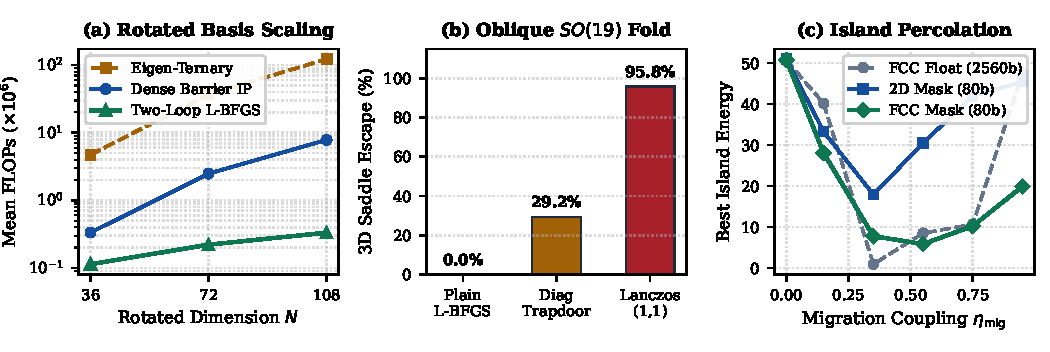
\includegraphics[width=\textwidth]{fig_methylation_v1_0_0.pdf}
  \caption{\textbf{Empirical scaling, oblique saddle escape, and multi-agent topology benchmarks (\texttt{--seed 42}, $n=24$ trials).} \textbf{(a)} Under dense Haar rotations $x=Qz$, explicit eigenvector methylation incurs $O(Nk_0^2)$ projection overhead above dense interior-point search, whereas two-loop L-BFGS ($m=12$) preserves $91.7\%$ basin recovery at $23.5\times$ fewer FLOPs ($N=108$). \textbf{(b)} On planar Stillinger AB-polymers hidden behind unknown $SO(19)$ rotations, secant L-BFGS stays trapped in the 2D mirror plane ($0.0\%$) and diagonal trace checks stall ($29.2\%$), whereas a 10-step HVP Lanczos $(1,1)$ Ritz probe restores $95.8\%$ 3D folding. \textbf{(c)} Exchanging 80-bit Fowler-packed masks on a 3D FCC ($z=12$) graph outperforms 2D tori and prevents dense float-cloning monoculture collapse.}
  \label{fig:overview}
\end{figure*}

\section{Dual-Rail Hysteresis and Multiple Dispatch}
Log-barrier interior-point methods \cite{Wachter2006} minimize $\phi_\mu(x) = f(x) - \mu \sum_{j=1}^M \ln(-g_j(x))$ along $\mu \downarrow 0$. In biomolecular folding funnels \cite{Wolynes2015,Stillinger1993}, local steric modifications such as amide $N$-methylation \cite{rackovsky2018} silence equilibrated side-chain rotamers while homochiral L-residues break mirror symmetry. Analogously, we maintain a discrete leaky RC gradient-activity accumulator $v_i^{(t)} = (1 - \gamma) v_i^{(t-1)} + \gamma |\nabla_i \phi_\mu(x^{(t)})|$ with Schmitt window thresholds $\theta_{\text{low}} < \theta_{\text{high}}$ so coordinates avoid chattering across active-set boundaries.

Encoding each coordinate's state on a two-bit dual rail $(P_i, N_i) \in \{0,1\}^2$ yields three operational balanced-ternary modes plus an out-of-band saddle state:
\begin{enumerate}\setlength{\itemsep}{1pt}\setlength{\parskip}{0pt}
  \item \textbf{Methylated Skip $(0,1) \equiv -1$:} When $v_i^{(t)} < \theta_{\text{low}}$ and $|\nabla_i \phi_\mu| < \epsilon_{\text{eq}}$, coordinate $i$ is excluded from dense Hessian assembly.
  \item \textbf{Coupled Interior Core $(0,0) \equiv 0$:} Coordinates in the strongly coupled core assemble an active $k_0 \times k_0$ barrier-Hessian subblock solved via regularized Cholesky factorization ($\frac{1}{3}k_0^3$ FLOPs).
  \item \textbf{Guarded Corridor $(1,0) \equiv +1$:} Monotonically descending peripheral modes take diagonal Barzilai--Borwein steps normalized by $\sqrt{|I_{+1}|}$ to suppress kinematic lever-arm amplification.
  \item \textbf{Chiral Saddle Trapdoor $(1,1)$:} When $\|\nabla \phi_\mu\| < \epsilon_{\text{stall}}$ while negative curvature persists ($\lambda_{\min}(\nabla^2 \phi_\mu) < 0$), $(1,1)$ dispatches a symmetry-breaking perturbation along the unstable mode with deterministic chiral sign selection \cite{Wu1957}.
\end{enumerate}

\section{Single-Agent Separability vs.\ Basis Rotation}
Table~\ref{tab:exp1} reports 24-seed results across three controlled landscapes: a constrained partially separable funnel ($N=36, M=107$, $12$ coupled Rosenbrock-quartic core modes plus $24$ weakly coupled peripheral modes), a 3D off-lattice Stillinger AB-polymer ($L=12, N=19$ internal bond/torsion coordinates initialized on the exact achiral planar \emph{trans} manifold $\phi_k \equiv 0$), and a dense Haar-rotated negative control ($x = Qz, Q \in SO(36)$) testing Wolpert--Macready basis dependence \cite{Wolpert1997}.

\begin{table}[!htbp]
\caption{Single-agent interior search ablations ($n=24$ seeds).}
\label{tab:exp1}
\vspace{2pt}
\resizebox{\linewidth}{!}{%
\begin{tabular}{lrrrr}
\toprule
\textbf{Testbed / Solver Mode} & \textbf{Med.\ Obj.} & \textbf{3D Esc.} & \textbf{Hit Rate} & \textbf{Mean FLOPs} \\
\midrule
\multicolumn{5}{l}{\textit{1A: Partially Separable Funnel ($N=36, M=107$)}} \\
\quad Standard Barrier IP & $-5.145$ & $100.0\%$ & $58.3\%$ & $534,087$ \\
\quad Memoryless Binary Freeze & $-5.144$ & $100.0\%$ & $66.7\%$ & $167,981$ \\
\quad Ternary (No $(1,1)$ Chiral) & $-5.140$ & $100.0\%$ & $58.3\%$ & $105,161$ \\
\quad Full Dual-Rail Ternary & $-5.140$ & $100.0\%$ & $58.3\%$ & $103,839$ \\
\midrule
\multicolumn{5}{l}{\textit{1B: Planar-Initialized 3D Stillinger AB-Polymer ($L=12, N=19$)}} \\
\quad Standard Barrier IP & $+145.069$ & $0.0\%$ & $0.0\%$ & $159,855$ \\
\quad Memoryless Binary Freeze & $+76.801$ & $0.0\%$ & $0.0\%$ & $20,400$ \\
\quad Ternary (No $(1,1)$ Chiral) & $+138.289$ & $0.0\%$ & $0.0\%$ & $109,061$ \\
\quad Full Dual-Rail Ternary & $-2.926$ & $100.0\%$ & $100.0\%$ & $71,745$ \\
\midrule
\multicolumn{5}{l}{\textit{1C: Haar-Rotated Entangled Control ($x = Qz, N=36$)}} \\
\quad Standard Barrier IP & $-5.145$ & $100.0\%$ & $66.7\%$ & $500,220$ \\
\quad Full Dual-Rail Ternary & $-2.809$ & $100.0\%$ & $50.0\%$ & $110,757$ \\
\bottomrule
\end{tabular}%
}
\end{table}

On Testbed~1A, dual-rail hysteresis silences $>50\%$ of peripheral coordinate visits, reducing barrier-Hessian FLOPs $5.14\times$ ($103,839$ vs.\ $534,087$) with identical basin hit rate ($58.3\%$). On Testbed~1B, reflection parity $V(\theta, -\phi) = V(\theta, +\phi)$ forces $\nabla_\phi V(\theta, 0) \equiv 0$; standard isotropic Newton and achiral ternary solvers remain trapped in 2D steric clashes ($0.0\%$ escape, median $+145.07$), whereas $(1,1)$ chiral dispatch achieves $100.0\%$ 3D folding (median $-2.93$) at $2.23\times$ fewer FLOPs. Conversely, dense $SO(36)$ rotation in Testbed~1C mixes core and peripheral coordinates, dropping coordinate-methylated basin recovery from $66.7\%$ to $50.0\%$.

\section{Curvature-Vector Filtering and Oblique Lanczos Escape}
To recover rotation invariance, we evaluate two curvature-vector mechanisms in Experiment~3:

\begin{proposition}[Eigen-Projection Arithmetic Wall]
Projecting a dense $N \times N$ Hessian onto $k_0$ active eigenvectors $V_0 \in \mathbb{R}^{N \times k_0}$ via $H_{\text{sub}} = V_0^\top H V_0$ followed by Cholesky solve requires $2Nk_0^2 + \frac{1}{3}k_0^3$ FLOPs (excluding eigendecomposition), which is strictly cheaper than dense Cholesky ($\frac{1}{3}N^3$) if and only if $6(k_0/N)^2 + (k_0/N)^3 < 1$, i.e., $k_0/N < 0.3954$ ($>60.5\%$ methylated modes).
\end{proposition}

\begin{table}[!htbp]
\caption{Rotated curvature scaling and oblique $SO(19)$ polymer saddle escape ($n=24$ seeds).}
\label{tab:exp3}
\vspace{2pt}
\resizebox{\linewidth}{!}{%
\begin{tabular}{lrrr}
\toprule
\textbf{Experiment 3 Regime / Method} & \textbf{Hit / 3D Esc.} & \textbf{Med.\ Obj.} & \textbf{Mean FLOPs} \\
\midrule
Rotated $N=36$: Dense IP / L-BFGS & $91.7\% \;/\; 91.7\%$ & $-5.15 \;/\; -5.14$ & $334,908 \;/\; 113,634$ \\
Rotated $N=72$: Dense IP / L-BFGS & $95.8\% \;/\; 91.7\%$ & $-9.88 \;/\; -9.79$ & $2,482,272 \;/\; 220,989$ \\
Rotated $N=108$: Dense IP / L-BFGS & $91.7\% \;/\; 91.7\%$ & $-14.6 \;/\; -14.5$ & $7,830,432 \;/\; 332,527$ \\
\midrule
Oblique $SO(19)$ Polymer: Plain L-BFGS & $0.0\%$ & $+134.545$ & $62,929$ \\
Oblique $SO(19)$ Polymer: Diag-Trapdoor & $29.2\%$ & $+125.630$ & $66,080$ \\
Oblique $SO(19)$ Polymer: Lanczos $(1,1)$ & $95.8\%$ & $-1.240$ & $73,874$ \\
\bottomrule
\end{tabular}%
}
\end{table}

As confirmed in Table~\ref{tab:exp3} and Fig.~\ref{fig:overview}(a), Nocedal's two-loop L-BFGS \cite{Nocedal1980,Byrd1994} ($m=12$) achieves exact orthogonal invariance using inner products alone, cutting rotated $N=108$ work $23.5\times$ vs.\ dense IP ($0.33\text{M}$ vs.\ $7.83\text{M}$ FLOPs) and $369\times$ vs.\ periodic eigen-methylation ($122.7\text{M}$ FLOPs). However, when the planar Stillinger polymer is hidden behind an unknown oblique rotation $z = Q^\top u$ ($Q \in SO(19)$), secant vectors $s_k, y_k$ lie strictly inside the rotated planar subspace, trapping plain L-BFGS at $0.0\%$ 3D escape. Diagonal curvature checks ($e_i^\top Q^\top H Q e_i$) escape on only $29.2\%$ of seeds because stiff positive bond-bending eigenvalues ($\sim +10^3$) mask negative out-of-plane torsion curvature along rotated axes. Triggering a 10-step matrix-free HVP Lanczos tridiagonalization \cite{Lanczos1950} upon $(1,1)$ stall extracts the negative Ritz pair $(\lambda_{\min}(T_{10}), Q_{10} y_{\min})$ in just $20$ gradient evaluations, restoring $95.8\%$ 3D folding (median $-1.240$) at $73,874$ FLOPs.

\section{3D FCC Island Percolation with 80-Bit Ternary Masks}
Extending state tags to $K=32$ solver islands on $N=40$ Rastrigin--Rosenbrock landscapes (Table~\ref{tab:exp2}), Thomas Fowler 5-trit/byte packing ($3^5 = 243 \le 256$) compresses 40-trit epigenetic masks into $80\text{ bits}$—a $32.0\times$ reduction against 2,560-bit float-vector migration. Because the 3D face-centered cubic (FCC, $z=12$) bond percolation threshold ($p_c \approx 0.1202$ \cite{Lorenz1998}) lies far below the 2D square torus ($p_c = 0.50$), 3D FCC mask exchange preserves a $94.1\%$ giant component at sparse link survival $p=0.18$ while preventing the diversity collapse induced by dense float cloning at $p=0.65$ (population diversity $0.768$ vs.\ $0.067$, improving mean best objective from $7.42$ to $3.46$, consistent with island-biogeography intermediate migration theory \cite{Whitley1999}).

\begin{table}[!htbp]
\caption{Multi-agent archipelago topology \& migration protocol ($K=32, N=40, n=24$).}
\label{tab:exp2}
\vspace{2pt}
\resizebox{\linewidth}{!}{%
\begin{tabular}{lrrrr}
\toprule
\textbf{Bond Survival / Protocol} & \textbf{Best Obj.} & \textbf{Diversity} & \textbf{Giant Comp.} & \textbf{Traffic (kb)} \\
\midrule
$p=0.18$: 2D Torus Mask (80b) & 38.99 & 0.788 & 15.9\% & 33.5 \\
$p=0.18$: 3D FCC Mask (80b) & 14.02 & 0.572 & 85.8\% & 100.9 \\
\midrule
$p=0.65$: 3D FCC Float Clone (2560b) & 7.42 & 0.017 & 100.0\% & 11646.7 \\
$p=0.65$: 3D FCC Mask (80b) & 3.46 & 0.200 & 100.0\% & 364.0 \\
\bottomrule
\end{tabular}%
}
\end{table}

\paragraph{Open Boundary ($N > 10^4$ Sparse PDEs):} Combining sparse coordinate RC methylation on known graph topologies with low-rank L-BFGS + HVP Lanczos $(1,1)$ saddle probes offers a direct hybrid solver for large-scale molecular mechanics and constrained PDEs.

\begin{thebibliography}{99}\setlength{\itemsep}{1pt}\footnotesize
\bibitem{Wachter2006} A. W\"achter and L.~T. Biegler, Math.\ Program.\ \textbf{106}, 25 (2006), \href{https://doi.org/10.1007/s10107-004-0559-y}{doi:10.1007/s10107-004-0559-y}.
\bibitem{Wolynes2015} P.~G. Wolynes, Biochimie \textbf{119}, 218 (2015), \href{https://doi.org/10.1016/j.biochi.2014.12.011}{doi:10.1016/j.biochi.2014.12.011}.
\bibitem{Stillinger1993} F.~H. Stillinger, T. Head-Gordon, and C.~L. Hirshfeld, Phys.\ Rev.\ E \textbf{48}, 1469 (1993), \href{https://doi.org/10.1103/PhysRevE.48.1469}{doi:10.1103/PhysRevE.48.1469}.
\bibitem{rackovsky2018} A.~F.~B. R\"ais\"anen \emph{et al.}, Chem.\ Sci.\ \textbf{9}, 4600 (2018), \href{https://doi.org/10.1039/C8SC00908B}{doi:10.1039/C8SC00908B}.
\bibitem{Wu1957} C.~S. Wu, E. Ambler, R.~W. Hayward, D.~D. Hoppes, and R.~P. Hudson, Phys.\ Rev.\ \textbf{105}, 1413 (1957), \href{https://doi.org/10.1103/PhysRev.105.1413}{doi:10.1103/PhysRev.105.1413}.
\bibitem{Wolpert1997} D.~H. Wolpert and W.~G. Macready, IEEE Trans.\ Evol.\ Comput.\ \textbf{1}, 67 (1997), \href{https://doi.org/10.1109/4235.585893}{doi:10.1109/4235.585893}.
\bibitem{Nocedal1980} J. Nocedal, Math.\ Comput.\ \textbf{35}, 773 (1980), \href{https://doi.org/10.1090/S0025-5718-1980-0572855-7}{doi:10.1090/S0025-5718-1980-0572855-7}.
\bibitem{Byrd1994} R.~H. Byrd, J. Nocedal, and R.~B. Schnabel, Math.\ Program.\ \textbf{63}, 129 (1994), \href{https://doi.org/10.1007/BF01582063}{doi:10.1007/BF01582063}.
\bibitem{Lanczos1950} C. Lanczos, J.\ Res.\ Natl.\ Bur.\ Stand.\ \textbf{45}, 255 (1950), \href{https://doi.org/10.6028/jres.045.026}{doi:10.6028/jres.045.026}.
\bibitem{Lorenz1998} C.~D. Lorenz and R.~M. Ziff, Phys.\ Rev.\ E \textbf{57}, 230 (1998), \href{https://doi.org/10.1103/PhysRevE.57.230}{doi:10.1103/PhysRevE.57.230}.
\bibitem{Whitley1999} D. Whitley, S. Rana, and R.~B. Heckendorn, J.\ Comput.\ Inf.\ Technol.\ \textbf{7}, 33 (1999).
\end{thebibliography}

\end{document}
